\chapter{Python程式碼}
\section{Wali}

\begin{minipage}{\textwidth}
  \centering
  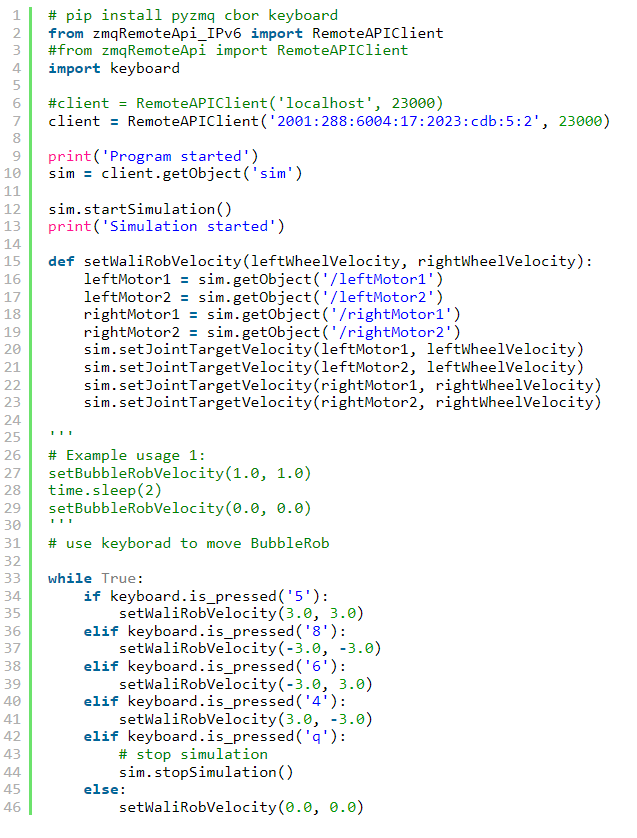
\includegraphics[width=\textwidth]{wali程式碼}
  \captionof{figure}{wali程式碼}
  \label{fig:wali程式碼}
\end{minipage}

\section{4輪BubbleRob}
因為發現原有Wali機器人結構太複雜,放8隻機器人會導致操控上很延遲,所以將4隻改成PJ1和PJ2的BubbleRob改良成4個輪子,以下為程式碼。\\

\begin{minipage}{\textwidth}
  \centering
  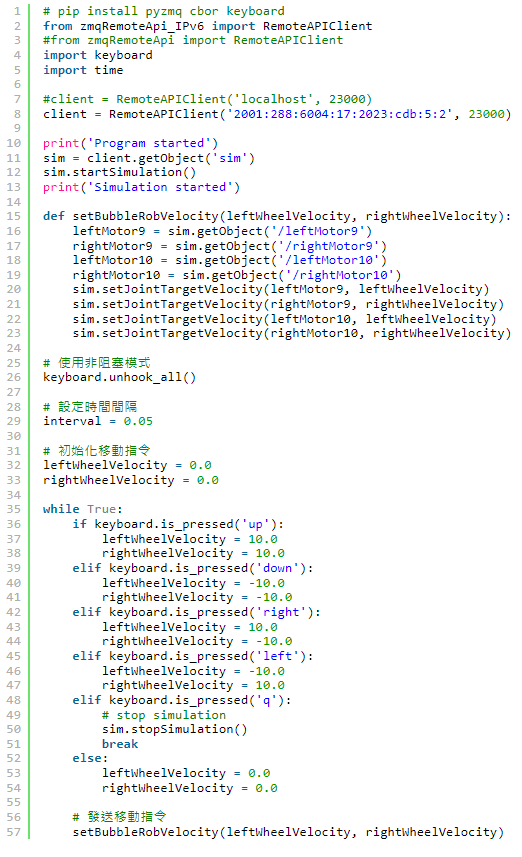
\includegraphics[width=0.5\textwidth]{4輪BubbleRob程式碼}
  \captionof{figure}{四輪BubbleRob程式碼}
  \label{fig:4輪BubbleRob程式碼}
\end{minipage}

\section{記分板}

\begin{minipage}{\textwidth}
  \centering
  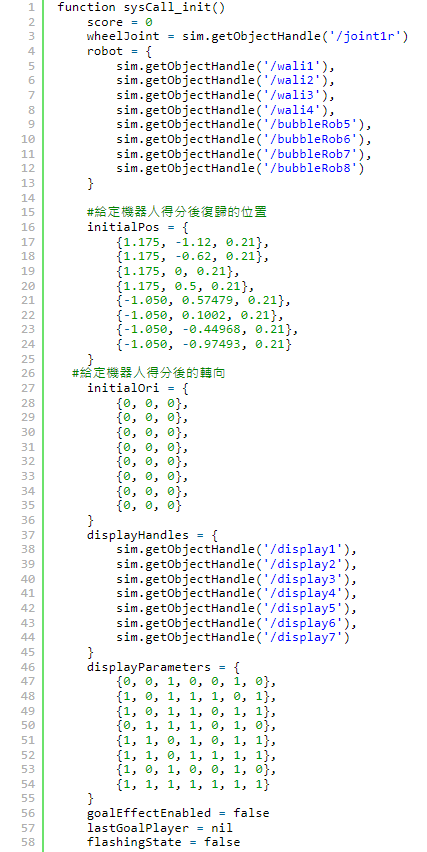
\includegraphics[width=0.5\textwidth]{記分板程式碼前半}
  \captionof{figure}{記分板程式碼前半}
  \label{fig:記分板程式碼前半}
\end{minipage}

\begin{minipage}{\textwidth}
  \centering
  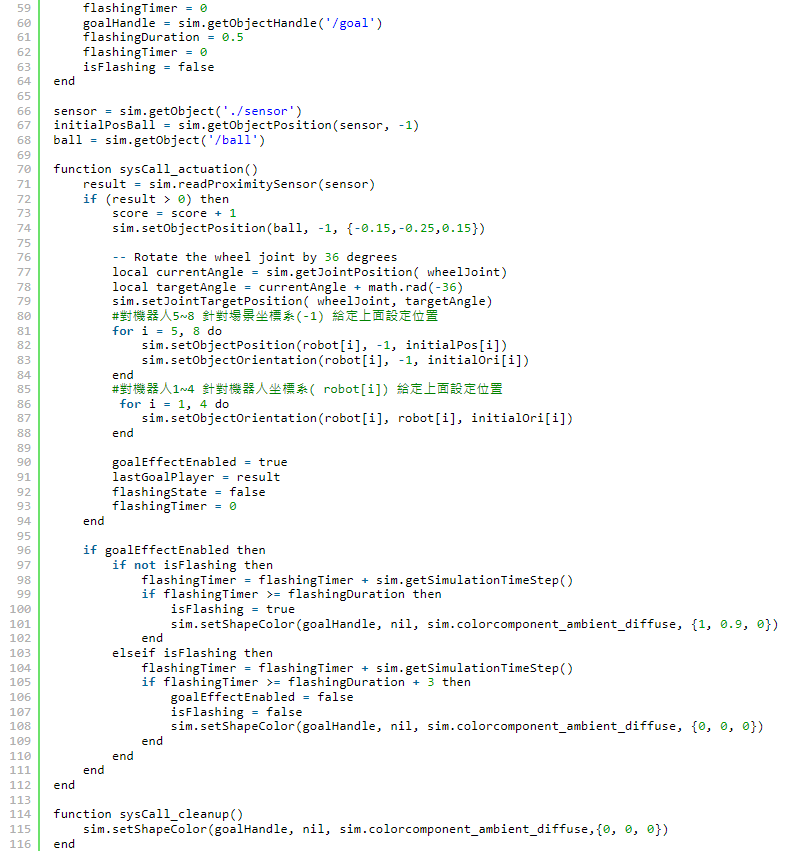
\includegraphics[width=0.5\textwidth]{記分板程式碼後半}
  \captionof{figure}{記分板程式碼後半}
  \label{fig:記分板程式碼後半}
\end{minipage}
\newpage
